% !Mode:: "TeX:UTF-8"
\chapter{插图}
\label{chap:figures}

插图主要涉及到:单个居中图形;两个并排图形;两个以上的并排或者堆叠的图形;图题;图形的引用;

\section{单个居中图形}

大多数情况下,需要插入的图形是单个的时候可以使用如下环境:

\begin{verbatim}
\begin{figure}[hptb]
 \centering
 
\includegraphics[width=6cm]{ysulogo}
 \caption{单个居中图形}\label{ysulogo}
\end{figure}
\end{verbatim}

其中的参数“[width=6cm]”指定图形的宽度6 cm。最后的效果如图\ref{ysulogo}所示。
\begin{figure}[hptb]
 \centering
 
\includegraphics[width=6cm]{ysulogo}
 \caption{单个居中图形}\label{ysulogo}
\end{figure}

\section{两个并排图形}
下列代码在文中插入两个并排的图形。它使用了一个称作minipage
的环境。在同一行插入两个并排的minipage,每个minipage包含一
个图形。图中minipage的参数“[0.5$\backslash$linewidth]”指定minipage
的宽度是当前正文页面的0.5倍(一半)。而插图命令中的参数
“[width=$\backslash$textwidth]”则是指定插图的宽度为当前minipage的宽
度。如果这个插图命令是在minipage环境外边的话,参数中的
“$\backslash$textwidth”的宽度为当前正文页面的宽度。
\begin{verbatim}
\begin{figure}[hptb]
  \centering
  \begin{minipage}[t]{0.5\linewidth}
    \centering
    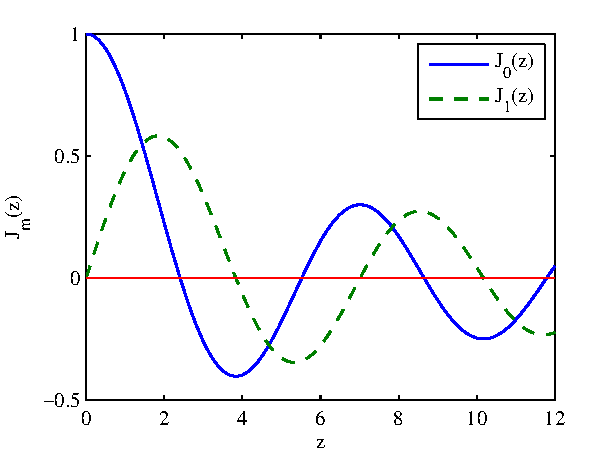
\includegraphics[width=\textwidth]{chp-2_bessel_j}
  \end{minipage}%
  \begin{minipage}[t]{0.5\textwidth}
    \centering
    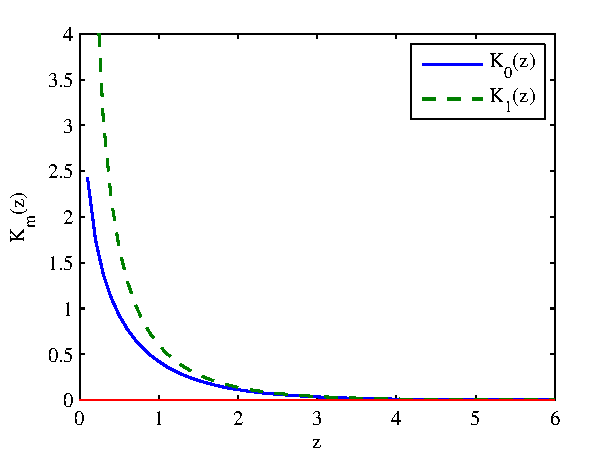
\includegraphics[width=\textwidth]{chp-2_bessel_k}
  \end{minipage}
    \caption{两个并排图形}\label{fig-dbfig}
\end{figure}
\end{verbatim}
最终结果如图\ref{fig-dbfig}所示。
\begin{figure}[hptb]
  \centering
  \begin{minipage}[t]{0.5\linewidth}
    \centering
    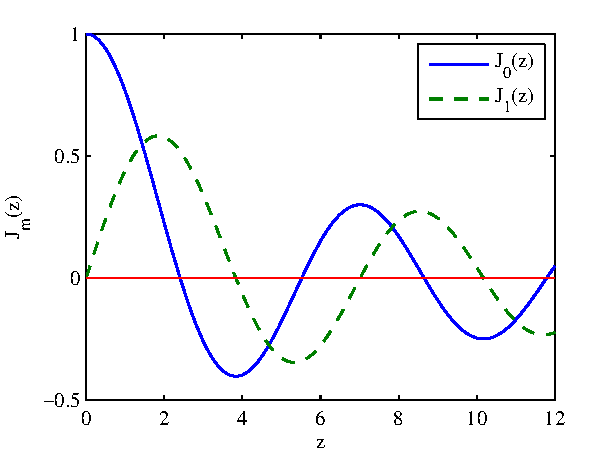
\includegraphics[width=\textwidth]{chp-2_bessel_j}
  \end{minipage}%
  \begin{minipage}[t]{0.5\textwidth}
    \centering
    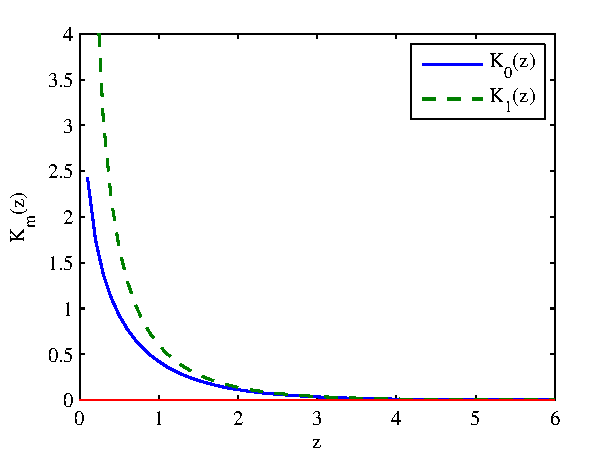
\includegraphics[width=\textwidth]{chp-2_bessel_k}
  \end{minipage}
    \caption{两个并排图形}\label{fig-dbfig}
 \end{figure}

\section{两个以上的并排或者堆叠的图形}
同样是使用minipage的方法,只不过排列的方式不同。例如4幅堆叠排列的图形。
\begin{verbatim}
\begin{figure}[hptb]
  \centering
  \begin{minipage}[t]{0.5\linewidth}
    \centering
    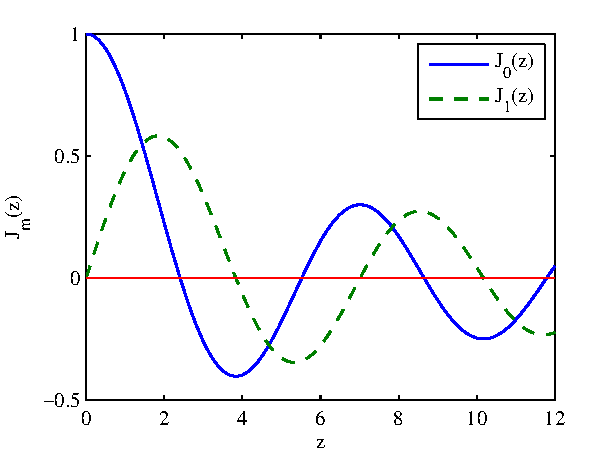
\includegraphics[width=\textwidth]{chp-2_bessel_j}
  \end{minipage}%
  \begin{minipage}[t]{0.5\textwidth}
    \centering
    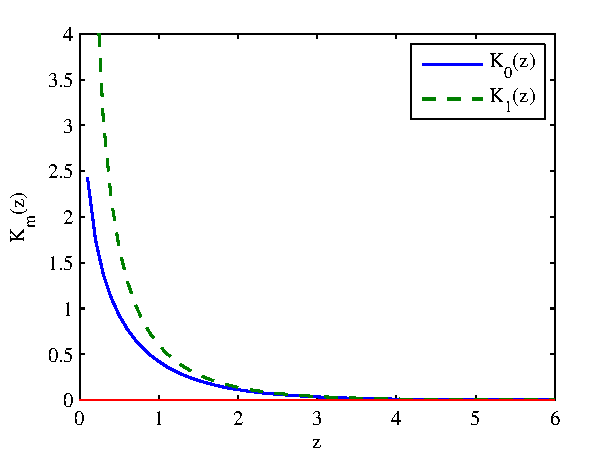
\includegraphics[width=\textwidth]{chp-2_bessel_k}
  \end{minipage}  \\
  \begin{minipage}[t]{0.5\textwidth}
    \centering
    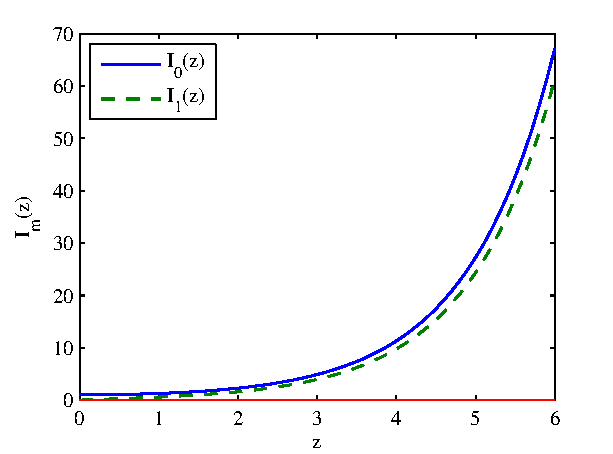
\includegraphics[width=\textwidth]{chp-2_bessel_i}
  \end{minipage}%
  \begin{minipage}[t]{0.5\textwidth}
    \centering
    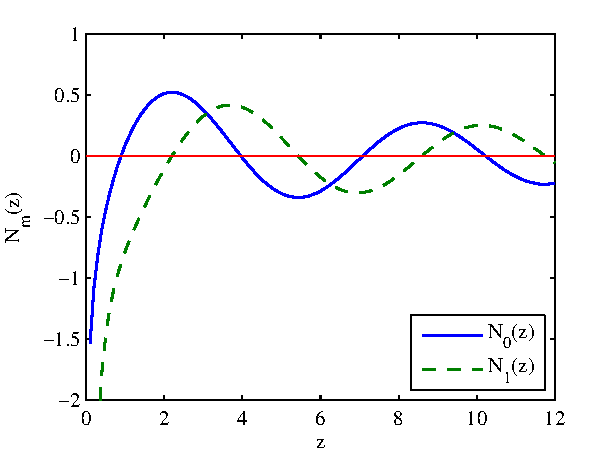
\includegraphics[width=\textwidth]{chp-2_bessel_n}
  \end{minipage}
\caption{贝塞尔函数}  \label{fig-bessel-function}
\end{figure}
\end{verbatim}
注意其中与一对并排图形不同的地方,加入了换行命令“$\backslash\backslash$”。
最终效果如图\ref{fig-bessel-function}所示。
\begin{figure}[hptb]
  \centering
  \begin{minipage}[t]{0.5\linewidth}
    \centering
    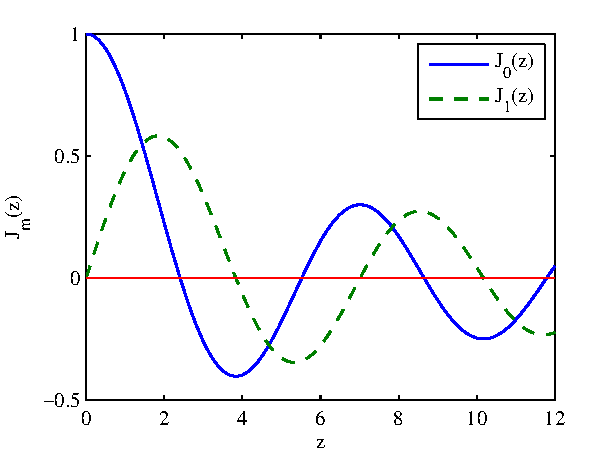
\includegraphics[width=\textwidth]{chp-2_bessel_j}
  \end{minipage}%
  \begin{minipage}[t]{0.5\textwidth}
    \centering
    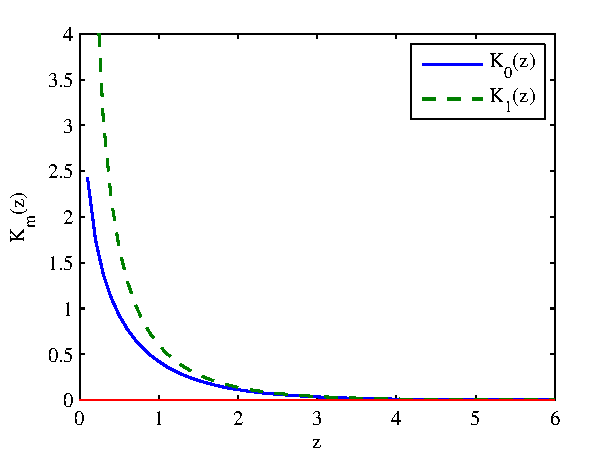
\includegraphics[width=\textwidth]{chp-2_bessel_k}
  \end{minipage}  \\
  \begin{minipage}[t]{0.5\textwidth}
    \centering
    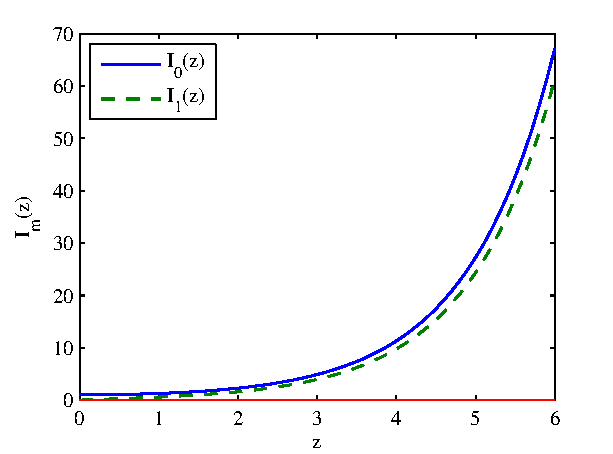
\includegraphics[width=\textwidth]{chp-2_bessel_i}
  \end{minipage}%
  \begin{minipage}[t]{0.5\textwidth}
    \centering
    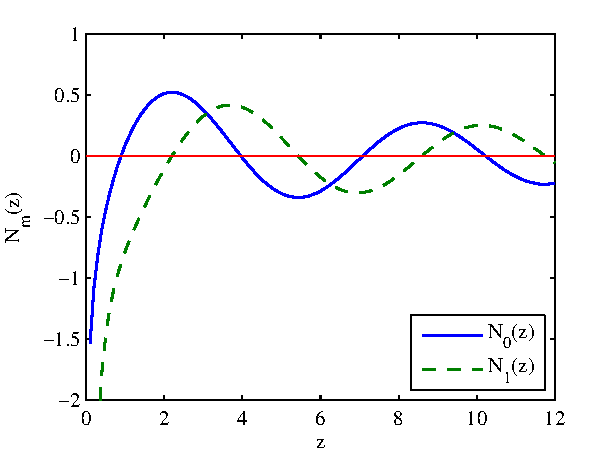
\includegraphics[width=\textwidth]{chp-2_bessel_n}
  \end{minipage}
\caption{贝塞尔函数}  \label{fig-bessel-function}
\end{figure}
其它类似的多个图形并排或者堆叠均可以灵活的运用minipage照猫画虎获得。

\section{图题}
其实上边的例子中已经包含了图题的引用命令\verb|\caption|。
例如图\ref{fig-bessel-function}中:
\begin{verbatim}
    \caption{贝塞尔函数}\label[fig-bessel-function]
\end{verbatim}
为当前的图形添加中文图题“贝塞尔函数”。同时添加标签“fig-bessel-function”。对图形的引用就是通过标签来实现的。

\section{图形的引用}
在已知图形的标签的基础之上,通过命令:
\begin{verbatim}
\ref{label}
\end{verbatim}
来引用标签为“label”的图形。\LaTeX 会自动将其替换为图形的编号。例如:
\begin{verbatim}
贝塞尔函数的图形如图\ref{fig-bessel-function}所示。
\end{verbatim}
的效果如下:\\
贝塞尔函数的图形如图\ref{fig-bessel-function}所示。
